\documentclass{article}
\usepackage{tikz}
\usetikzlibrary{fit,positioning}

\begin{document}


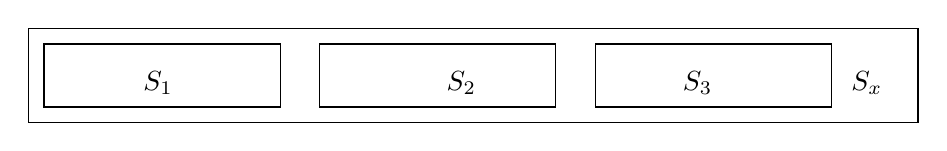
\begin{tikzpicture}[shift={(1,1)},local bounding box=A]
\draw (0,0) rectangle (11.3,1.2);
\draw (0.2,0.2) rectangle (3.2,1);
\draw (3.7,0.2) rectangle (6.7,1);
\draw (7.2,0.2) rectangle (10.2,1);
\node[scale=1] at (1.65,0.5) {$S_{1}$};
\node[scale=1] at (5.5,0.5) {$S_{2}$};
\node[scale=1] at (8.5,0.5) {$S_{3}$};
\node[scale=1] at (10.65,0.5) {$S_{x}$};
\end{tikzpicture}

{
.
\newline
\newline
\newline
}

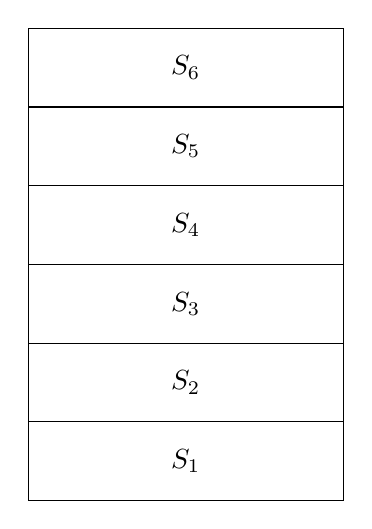
\begin{tikzpicture}
\draw (0,0) rectangle (4,6);

\draw (0,0) rectangle (4,1);
\draw (0,1) rectangle (4,1);
\draw (0,2) rectangle (4,1);
\draw (0,3) rectangle (4,1);
\draw (0,4) rectangle (4,1);
\draw (0,5) rectangle (4,1);
\draw (0,6) rectangle (4,1);


\node[scale=1] at (2,0.5) {$S_{1}$};
\node[scale=1] at (2,1.5) {$S_{2}$};
\node[scale=1] at (2,2.5) {$S_{3}$};
\node[scale=1] at (2,3.5) {$S_{4}$};
\node[scale=1] at (2,4.5) {$S_{5}$};
\node[scale=1] at (2,5.5) {$S_{6}$};
\end{tikzpicture}





{
.
\newline
\newline
\newline
}




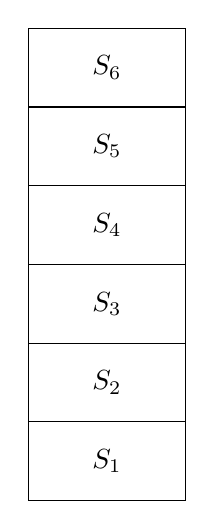
\begin{tikzpicture}
\draw (0,0) rectangle (2,6);

\draw (0,0) rectangle (2,1);
\draw (0,1) rectangle (2,1);
\draw (0,2) rectangle (2,1);
\draw (0,3) rectangle (2,1);
\draw (0,4) rectangle (2,1);
\draw (0,5) rectangle (2,1);
\draw (0,6) rectangle (2,1);


\node[scale=1] at (1,0.5) {$S_{1}$};
\node[scale=1] at (1,1.5) {$S_{2}$};
\node[scale=1] at (1,2.5) {$S_{3}$};
\node[scale=1] at (1,3.5) {$S_{4}$};
\node[scale=1] at (1,4.5) {$S_{5}$};
\node[scale=1] at (1,5.5) {$S_{6}$};
\end{tikzpicture}




{
.
\newline
\newline
\newline
}




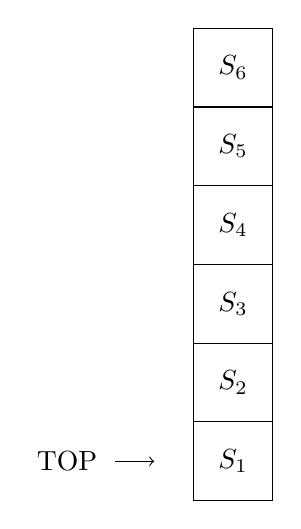
\begin{tikzpicture}
\draw (0,0) rectangle (1,6);

\draw (0,0) rectangle (1,1);
\draw (0,1) rectangle (1,1);
\draw (0,2) rectangle (1,1);
\draw (0,3) rectangle (1,1);
\draw (0,4) rectangle (1,1);
\draw (0,5) rectangle (1,1);
\draw (0,6) rectangle (1,1);

\draw [->] (-1,0.5) -- (-.5,0.5) node[left, xshift=-6mm] {TOP};


\node[scale=1] at (0.5,0.5) {$S_{1}$};
\node[scale=1] at (0.5,1.5) {$S_{2}$};
\node[scale=1] at (0.5,2.5) {$S_{3}$};
\node[scale=1] at (0.5,3.5) {$S_{4}$};
\node[scale=1] at (0.5,4.5) {$S_{5}$};
\node[scale=1] at (0.5,5.5) {$S_{6}$};
\end{tikzpicture}




{
.
\newline
\newline
\newline
}




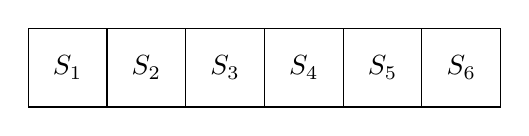
\begin{tikzpicture}
\draw (0,0) rectangle (6,1);

\draw (0,0) rectangle (1,1);
\draw (1,0) rectangle (1,1);
\draw (2,0) rectangle (1,1);
\draw (3,0) rectangle (1,1);
\draw (4,0) rectangle (1,1);
\draw (5,0) rectangle (1,1);
\draw (6,0) rectangle (1,1);


\node[scale=1] at (0.5,0.5) {$S_{1}$};
\node[scale=1] at (1.5,0.5) {$S_{2}$};
\node[scale=1] at (2.5,0.5) {$S_{3}$};
\node[scale=1] at (3.5,0.5) {$S_{4}$};
\node[scale=1] at (4.5,0.5) {$S_{5}$};
\node[scale=1] at (5.5,0.5) {$S_{6}$};
\end{tikzpicture}




{
.
\newline
\newline
\newline
}




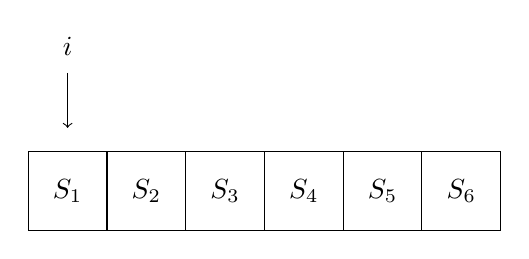
\begin{tikzpicture}
\draw (0,0) rectangle (6,1);

\draw (0,0) rectangle (1,1);
\draw (1,0) rectangle (1,1);
\draw (2,0) rectangle (1,1);
\draw (3,0) rectangle (1,1);
\draw (4,0) rectangle (1,1);
\draw (5,0) rectangle (1,1);
\draw (6,0) rectangle (1,1);

\draw [->] (0.5,2) -- (0.5,1.3) node[above, yshift=8mm] {$i$};

\node[scale=1] at (0.5,0.5) {$S_{1}$};
\node[scale=1] at (1.5,0.5) {$S_{2}$};
\node[scale=1] at (2.5,0.5) {$S_{3}$};
\node[scale=1] at (3.5,0.5) {$S_{4}$};
\node[scale=1] at (4.5,0.5) {$S_{5}$};
\node[scale=1] at (5.5,0.5) {$S_{6}$};
\end{tikzpicture}



\end{document}